\chapter{Parametric Exploration of the \emph{EvoTSC} Model}
\label{chap:param}

In this chapter, I present several sets of additional evolutionary simulations.
In these simulations, I explore the robustness of the characteristics of evolving populations to variations in the \emph{EvoTSC} model, measuring whether populations are able to evolve differentiated gene expression patterns as a response to different environments, and comparing their speed of evolution with that of the main runs presented in Chapter~\ref{chap:ploscb}.
I first explore changing different parameters, presented in Table~\ref{tab:param:params}: the maximum interaction distance for the transcription-supercoiling coupling, the mean intergenic distance, the strength of the environment-caused shift in background supercoiling, and the number of genes on the genome.
I then discuss the effect of introducing indels in intergenic sections as a new mutational operator in the model.

\begin{table}
\begin{center}
\begin{tabular}{l c r r}
\toprule
\textbf{Parameter} & \textbf{Symbol} & \textbf{Value} & \textbf{Replicates} \\
\midrule
Interaction distance & $d_{max}$ & \textbf{5 kb} & \textbf{30}\\
& & 25 kb & 15\\
\midrule
& & 10 bp& 15\\
Mean intergenic distance & $d_{mean}$ & \textbf{125 bp} & \textbf{30} \\
& & 1,000 bp & 15\\
& & 10,000 bp & 15 \\
\midrule
& & 0.0001 & 15\\
Environment supercoiling & $\delta\sigma_{A/B}$ & 0.001 & 15\\
& & \textbf{0.01} & \textbf{30}\\
\midrule
Number of genes & $n$ & \textbf{60} & \textbf{30} \\
& & 30 & 15 \\
\bottomrule
\end{tabular}
\end{center}
\caption[Table of parameter values explored in additional \emph{EvoTSC} simulations]{Table of the parameters and associated values explored in additional experiments (separated by horizontal lines).
For each experiment, the row in bold font corresponds to the parameter values used in the main run described in Chapter~\ref{chap:ploscb}, and is shown for reference.}
\label{tab:param:params}
\end{table}

\section{Interaction Distance}
\label{sec:param:inter25k}

The size of the topological domains of bacterial genomes, inside which DNA supercoils can freely propagate, has historically been estimated to be on the order of a few thousand base pairs~\citep{elhanafi2000,kouzine2013}.
Recent work has however suggested that topological domains could be up to ten times larger than this, reaching up to 25 kb~\citep{visser2022}.
As this distance sets a limit to the number of genes that can interact through the transcription-supercoiling coupling, it plays an important role in the structure of the supercoiling-mediated gene regulatory networks.
By increasing the number of genes a given gene is coupled with, a larger interaction distance could make genomic inversions more deleterious by making them disrupt a larger part of the regulatory networks at their boundaries, but could also allow more robust regulatory networks to evolve through a higher connectivity.
In this section, I present simulations run with an interaction distance of 25 kb, in order to test this hypothesis.

\begin{figure}[H]
\centering
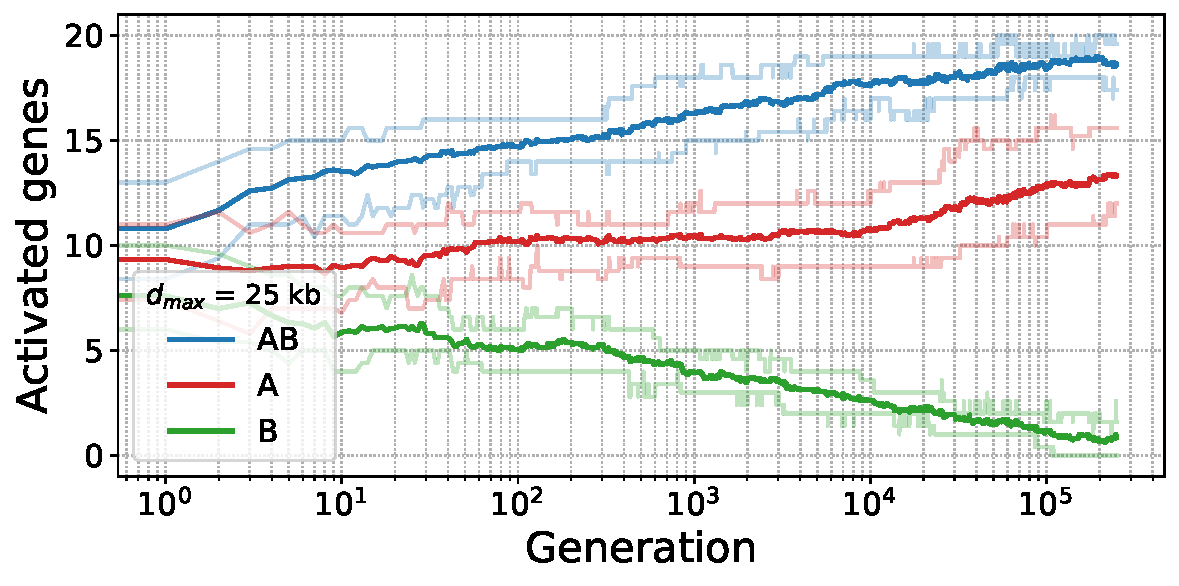
\includegraphics[width=0.495\textwidth]{param/interaction-25k/gene_activity_env_A.pdf}
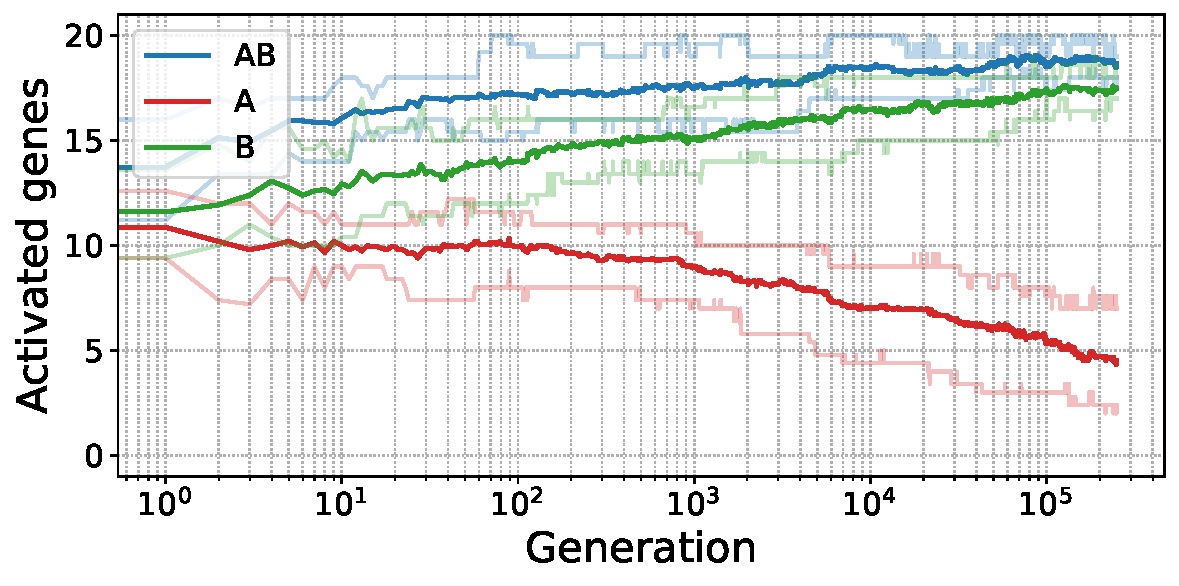
\includegraphics[width=0.495\textwidth]{param/interaction-25k/gene_activity_env_B.pdf}
\caption[Evolution of the number of activated genes in each environment, with an interaction distance of 25 kb]{Evolution of the number of activated genes in environment A (left) and environment B (right), with an interaction distance of 25 kb.}
\label{fig:param:inter25k-activ-by-env}
\end{figure}

Figure~\ref{fig:param:inter25k-activ-by-env} shows the evolution of the number of activated genes of each type in the simulations with the interaction distance of 25 kb, over 250,000 generations.
As in the main run, the number of activated genes of each type evolves towards their respective target.
Differentiated activation patterns can therefore still evolve even when the topological domains are 5 times larger.

\begin{figure}[H]
\centering
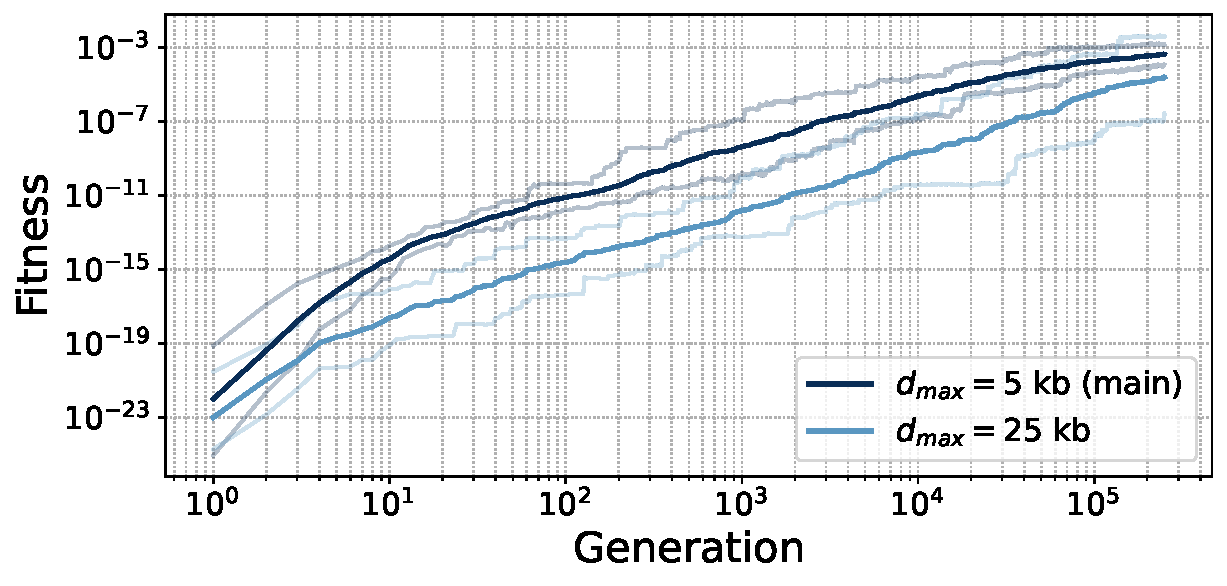
\includegraphics[width=0.75\textwidth]{param/interaction-25k/fitness_all_with_main.pdf}
\caption[Average fitness during evolution, with an interaction distance of 25 kb]{Average fitness during evolution with an interaction distance of 25 kb (yellow).
The main run is presented in purple for comparison.}
\label{fig:param:inter25k-fitness}
\end{figure}

Figure~\ref{fig:param:inter25k-fitness} shows the evolution of the average fitness of the best individual in each replicate of the simulation with a larger interaction distance, compared with the evolution of fitness in the main run, over 250,000 generations.
While fitness is systematically lower throughout evolution with the larger interaction distance, it nonetheless follows a qualitatively similar pattern, and fitness keeps increasing until the end of the runs, suggesting that it could eventually reach the same value as in the main run (presented in full in Figure~\ref{fig:ploscb:main_fitness}).

\begin{figure}[H]
\centering
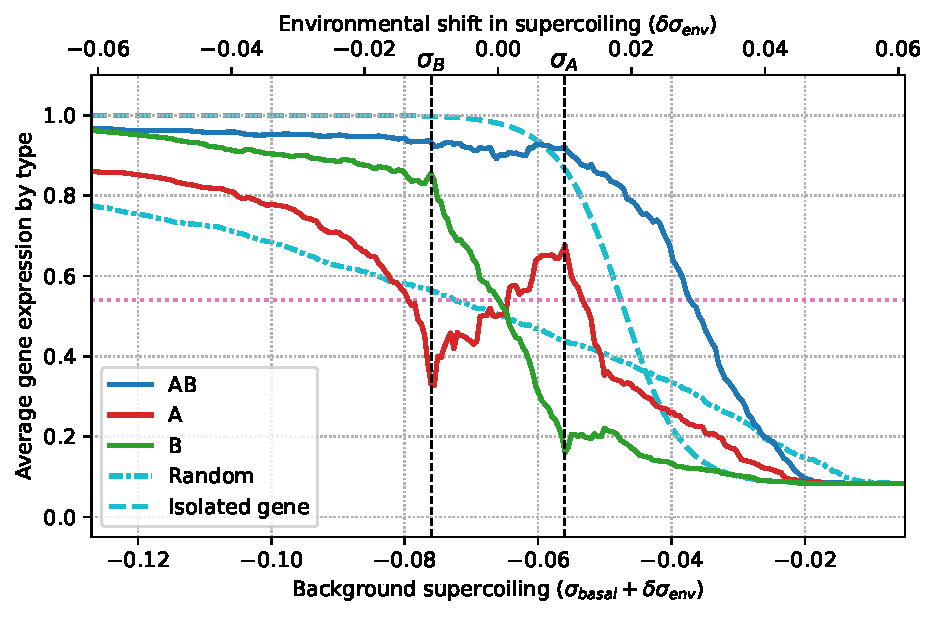
\includegraphics[width=0.9\textwidth]{param/interaction-25k/activity_sigmas_avg.pdf}
\caption[Average gene expression as a function of background supercoiling, with an interaction distance of 25 kb]{Average gene expression by type as a function of background supercoiling, with an interaction distance of 25 kb.
The dash-dotted line represents the average expression of genes on a random genome with an interaction distance of 25 kb.}
\label{fig:param:inter25k-activ-by-sigma}
\end{figure}

Figure~\ref{fig:param:inter25k-activ-by-sigma} shows the average gene expression by type of evolved individuals, as a function of the background supercoiling level.
As in the main run, \emph{A} genes display a relaxation-activated phenotype.
\emph{AB} and \emph{B} genes are relaxation-inhibited, but nonetheless display quite different behaviors than the (dash-dotted light blue) curve for genes on a random genome with the same parameters, which present a much flatter response curve to background supercoiling than with the default interaction distance of 5 kb (shown in Figure~\ref{fig:ploscb:activity_by_sigma}).

\begin{figure}[H]
\centering
  \begin{subfigure}[t]{0.495\textwidth}
    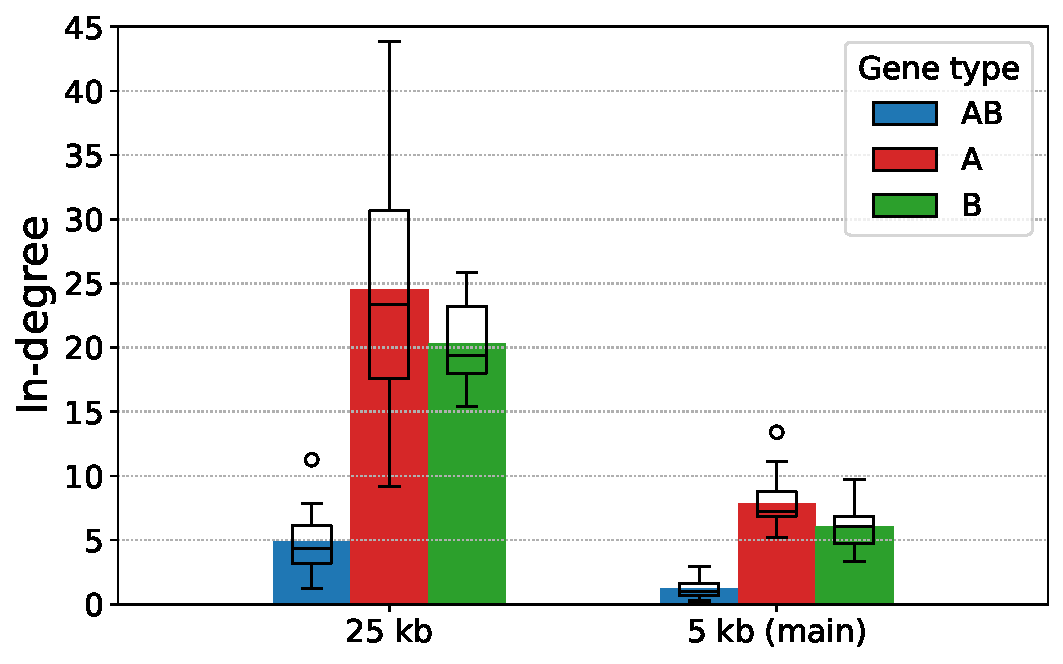
\includegraphics[width=\textwidth]{param/interaction-25k/effective_graph_combined_in_degree.pdf}
  \end{subfigure}
  \begin{subfigure}[t]{0.495\textwidth}
    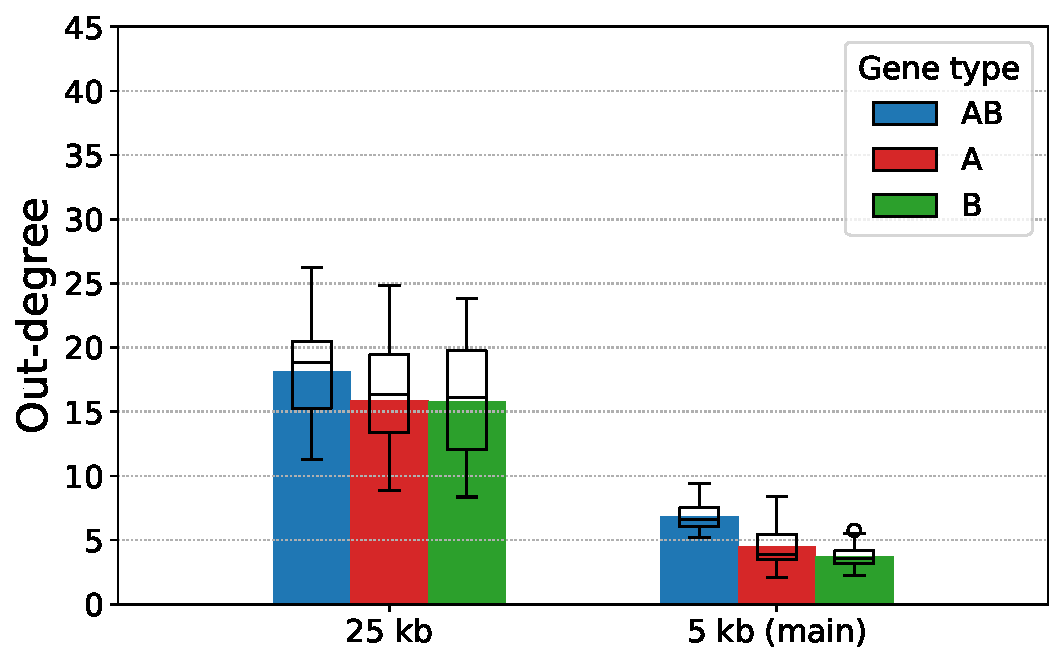
\includegraphics[width=\textwidth]{param/interaction-25k/effective_graph_combined_out_degree.pdf}
  \end{subfigure}
  \caption[Average in- and out-degree of effective interaction graph nodes, with an interaction distance of 25 kb]{Average out-degree (left) and in-degree (right) of the genes in the effective interaction graph, separated by gene type, for individuals with an interaction distance of 5 kb (main run) or 25 kb.}
  \label{fig:param:inter25k-degree}
\end{figure}

Figure~\ref{fig:param:inter25k-degree} finally presents the average in- and out-degree of the genes in the effective interaction graph obtained with gene knockouts, compared to the same data from the main run.
As could be expected, the gene regulatory networks are much more connected with the larger interaction distance, but the behavior per gene type remains qualitatively the same as in the main run.


\section{Mean Intergenic Size}
\label{sec:param:mean-intergene}

In the main run, I set the initial intergenic distance between every gene to 125 bp, or a gene density of 88\%, representing the average \emph{E. coli} intergenic distance~\citep{postow2004}, but bacteria actually present a wider range of gene densities~\citep{kuo2009}.
Like the interaction distance, the mean intergenic distance plays a role in the connectivity of the gene regulatory networks that stem from the transcription-supercoiling coupling: the smaller the mean intergenic distance, the more genes can interact.
Conversely, when the mean intergenic distance is large compared to the interaction distance, the emergence of regulatory networks isolated from each other by large intergenic regions becomes possible.
In this chapter, I present simulations with mean intergenic distances increasing logarithmically from 10 bp (or a gene density of 99\%) to 10 kb (or a gene density of 10\%), representing gene-scarce eukaryotic genomes~\citep{davilalopez2010}, in order to test the robustness of the results with regard to the range of gene densities found across living organisms.

\begin{figure}[H]
\centering
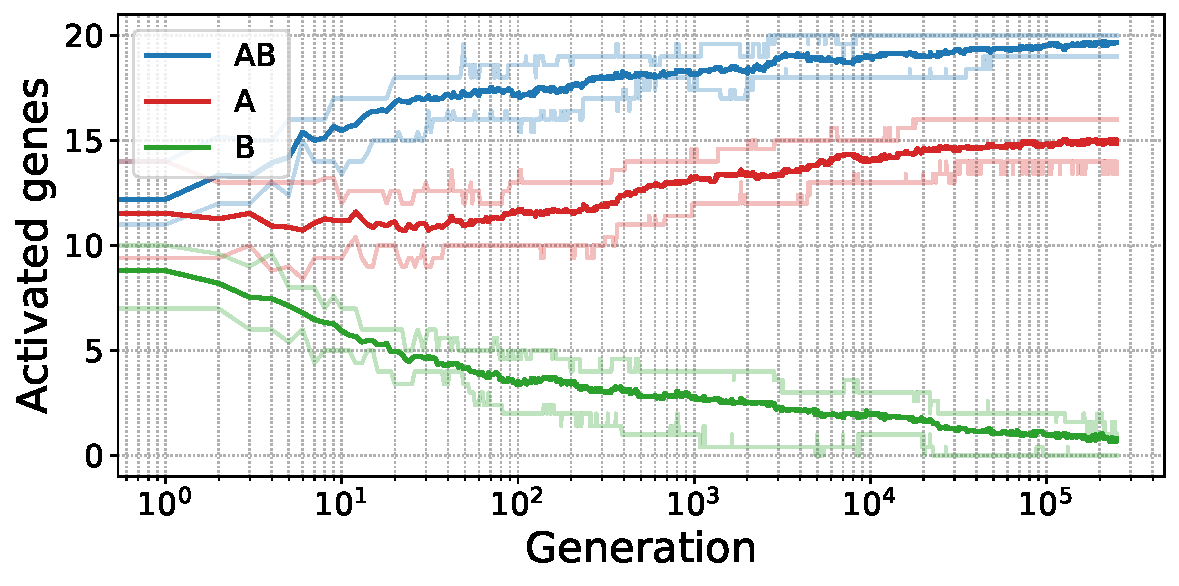
\includegraphics[width=0.495\textwidth]{param/mean-intergene/inter-0.01k/gene_activity_env_A.pdf}
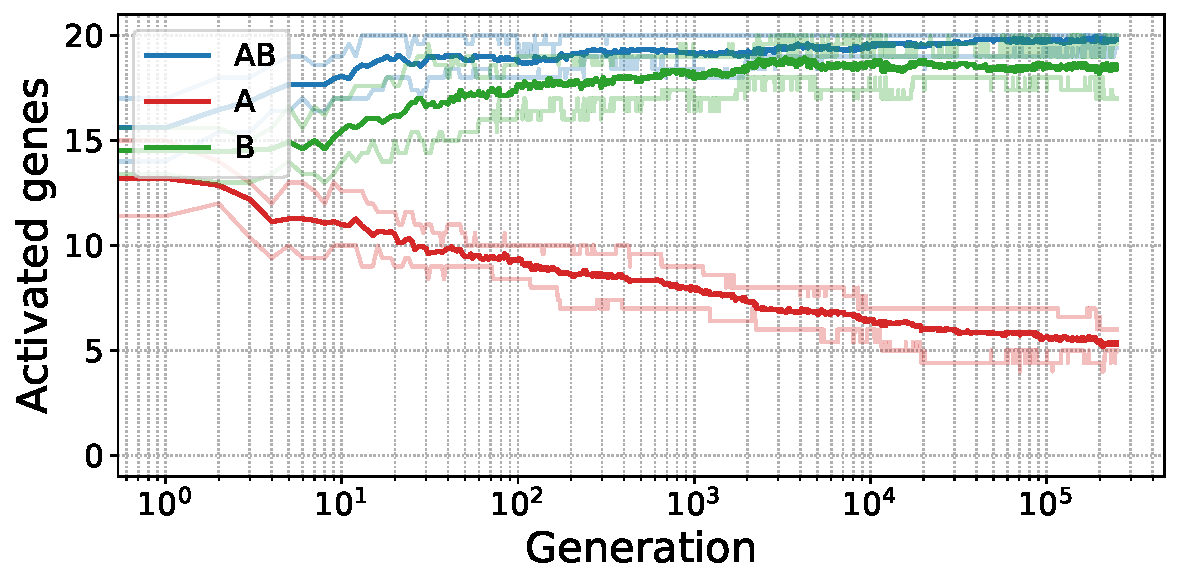
\includegraphics[width=0.495\textwidth]{param/mean-intergene/inter-0.01k/gene_activity_env_B.pdf}

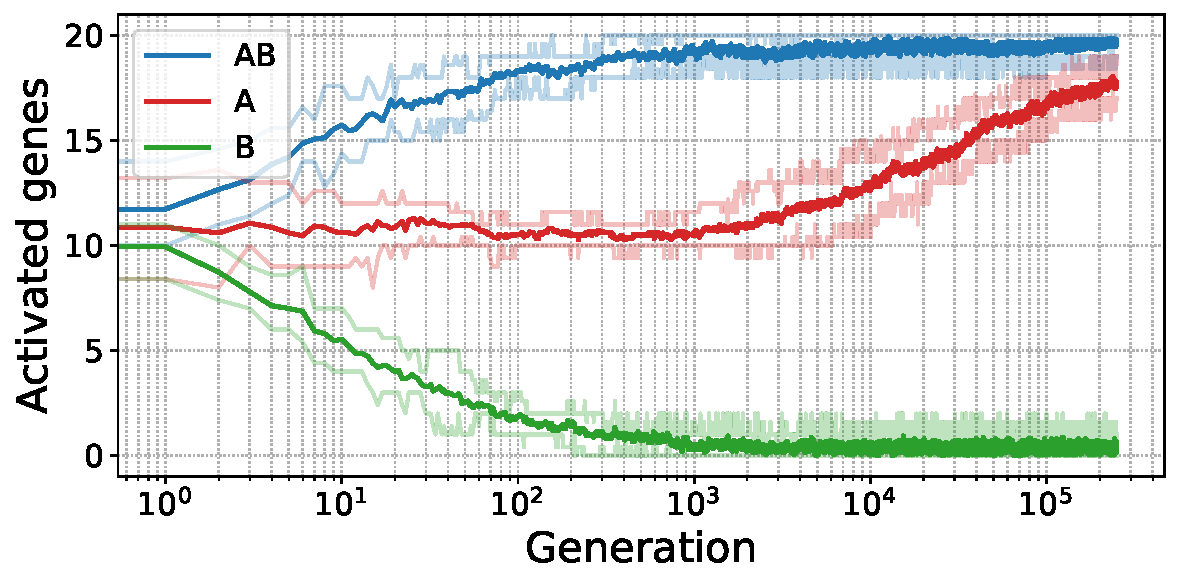
\includegraphics[width=0.495\textwidth]{param/mean-intergene/inter-1k/gene_activity_env_A.pdf}
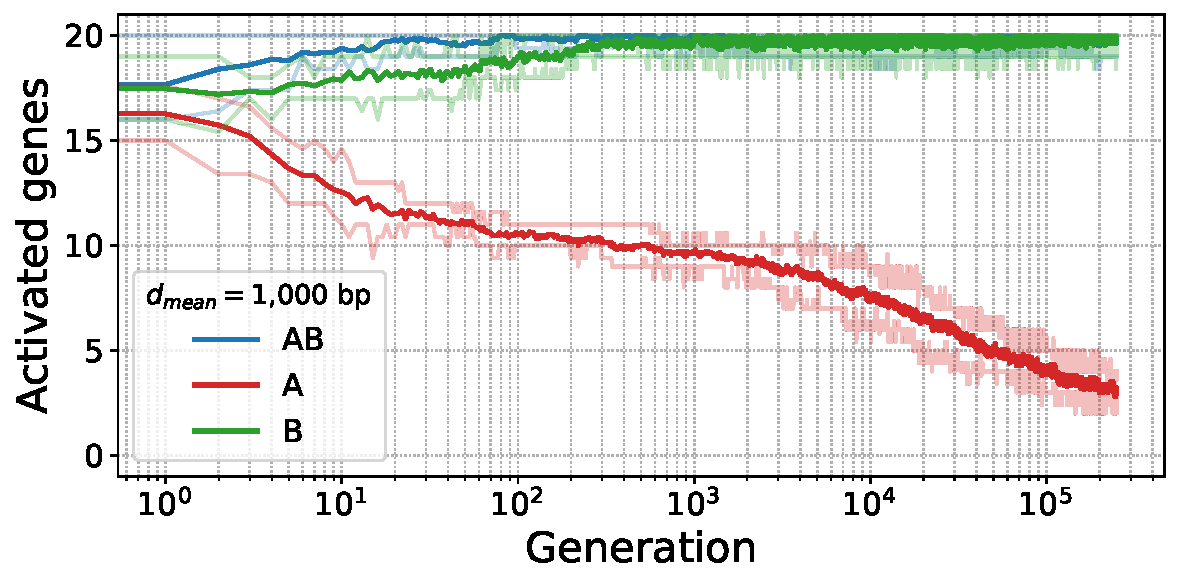
\includegraphics[width=0.495\textwidth]{param/mean-intergene/inter-1k/gene_activity_env_B.pdf}

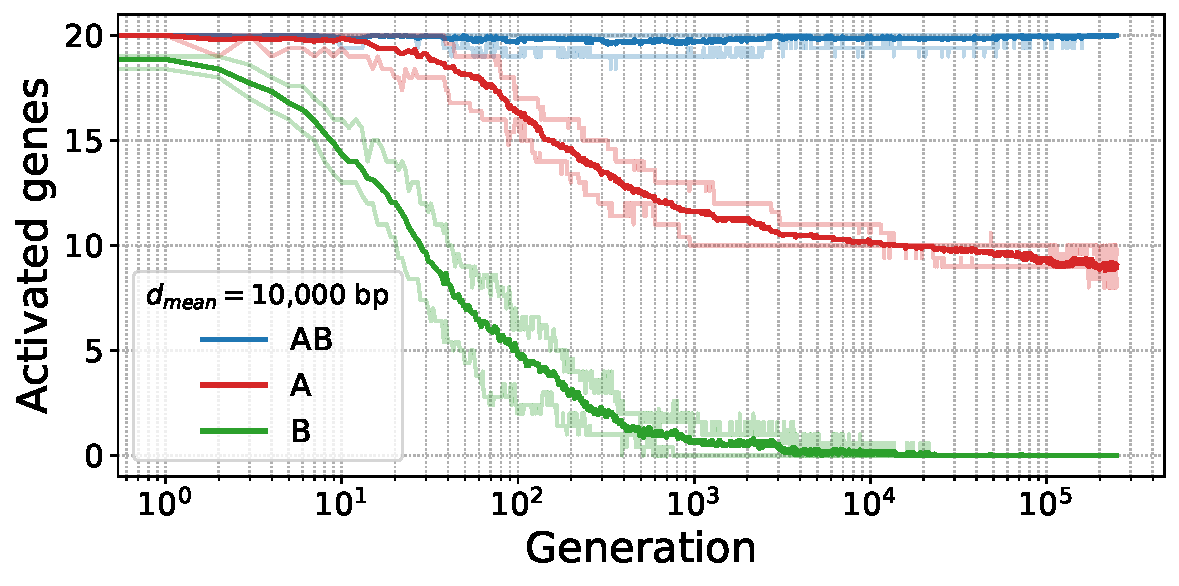
\includegraphics[width=0.495\textwidth]{param/mean-intergene/inter-10k/gene_activity_env_A.pdf}
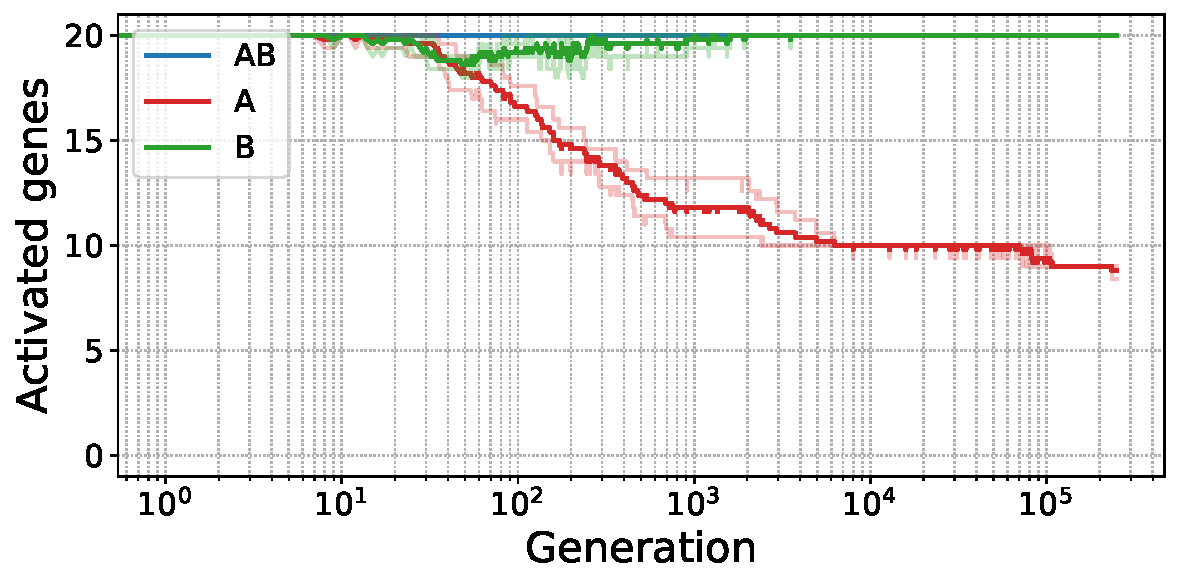
\includegraphics[width=0.495\textwidth]{param/mean-intergene/inter-10k/gene_activity_env_B.pdf}
\caption[Evolution of the number of activated genes in each environment, with increasing mean intergenic distances]{Average number of activated genes per gene type in environment A (left) and B (right) during evolution, for average intergenic sizes of 10 bp (top), 1 kb (middle), and 10 kb (bottom).}
\label{fig:param:mean-intergene-activ-by-env}
\end{figure}

Figure~\ref{fig:param:mean-intergene-activ-by-env} shows the evolution of the number of activated genes for each gene type in each environment, with mean intergenic distances increasing from top to bottom, for 250,000 generations.
For intergenic distances of 10 bp and 1 kb, the number of activated genes converges towards the target in each environment, as in the main run.
For a mean intergenic distance of 10 kb, the behavior is different: while \emph{AB} genes and \emph{B} genes evolve towards the correct activation state in each environment, the proportion of activated \emph{A} genes stays close to 50\% in each environment, showing that \emph{A} genes do not evolve a differentiated expression pattern depending on the environment.

\begin{figure}
\centering
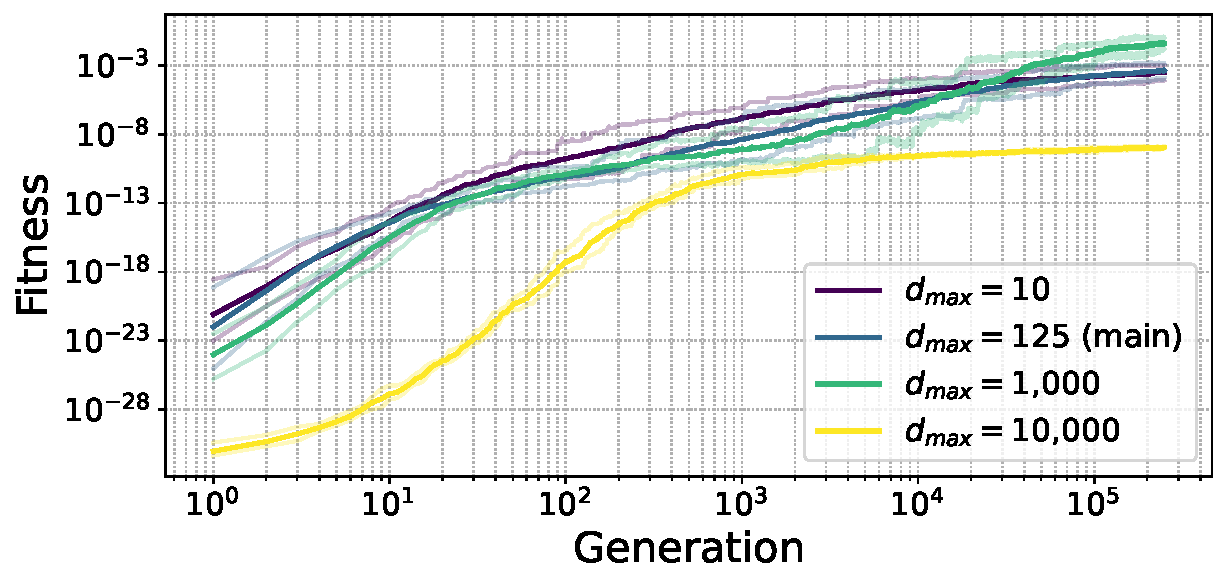
\includegraphics[width=0.75\textwidth]{param/mean-intergene/fitness_all_with_main.pdf}
\caption[Average fitness during evolution, with increasing mean intergenic distances]{Average fitness during evolution for average intergenic distances of 10 bp, 125 bp (main run), 1 kb, and 10 kb.}
\label{fig:param:mean-intergene-fitness}
\end{figure}

Figure~\ref{fig:param:mean-intergene-fitness} shows the evolution of the average fitness of the best individual in each replicate of the simulations, for each value of the mean intergenic distance, including the main run for comparison.
It confirms the results seen in the previous figure: for intergenic distances from 10 bp to 1 kb, populations evolve successfully towards differentiated gene activation patterns.
For an intergenic size of 10 kb (in yellow), however, fitness increases much more slowly, and seems to converge towards a much smaller value.

\begin{figure}
\centering
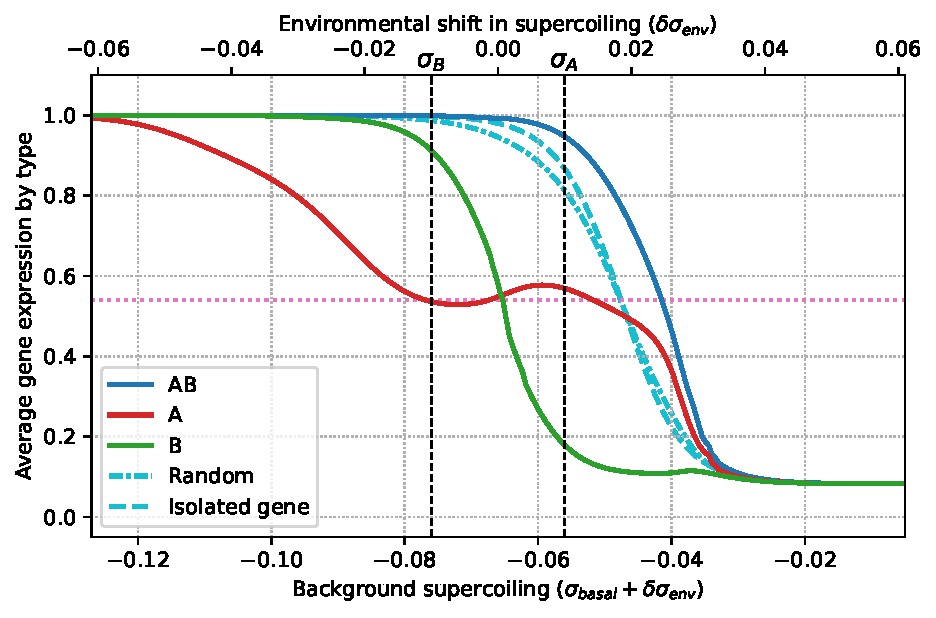
\includegraphics[width=0.9\textwidth]{param/mean-intergene/inter-10k/activity_sigmas_avg.pdf}
\caption[Average gene expression as a function of background supercoiling, with an intergenic distance of 10 kb]{Average gene expression as a function of background supercoiling, with an intergenic distance of 10 kb.}
\label{fig:param:mean-intergene-10kb-activ-by-sigma}
\end{figure}

Figure~\ref{fig:param:mean-intergene-10kb-activ-by-sigma} shows the average gene activity as a function of background supercoiling, for the best individual in each of the replicates with a mean intergenic distance of 10 kb.
In this case, we do not observe a relaxation-activated phenotype for \emph{A} genes as clearly as in the main simulation.
Instead, the average expression level of \emph{A} genes is indeed slightly lower in environment B than in environment A, but remains close to half expression for background supercoiling values between -0.08 and -0.05.

\begin{figure}
\centering
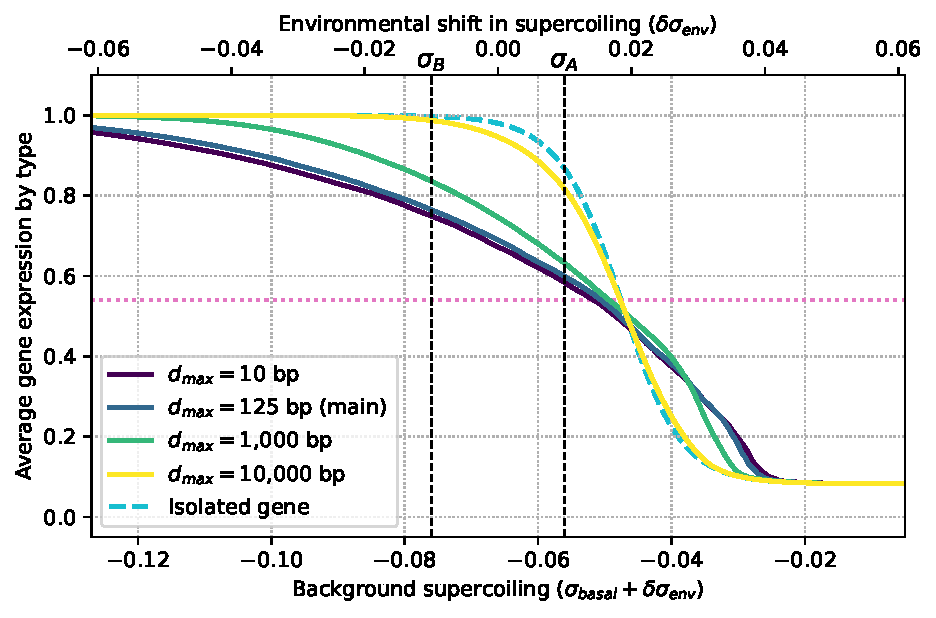
\includegraphics[width=0.9\textwidth]{param/mean-intergene/random_activ_per_sigma.pdf}
\caption[Average gene expression as a function of background supercoiling, with increasing mean intergenic distances, in random genomes]{Average gene expression as a function of background supercoiling in random genomes with different mean intergenic distances (full lines), and theoretical expression level of an isolated gene (dashed line).}
\label{fig:param:mean-intergene-random-activ-by-sigma}
\end{figure}

Figure~\ref{fig:param:mean-intergene-random-activ-by-sigma} shows the expression level as a function of background supercoiling for genes on random genomes with increasing mean intergenic distances.
For distances from 10 bp to 1 kb, the curve is qualitatively similar, and quite different to the expression of an isolated, non-interacting genes.
In particular, gene expression levels are sensibly lower than the maximum in both environment A and environment B.
On the other hand, for a mean intergenic distance of 10 kb (in yellow), genes on average behave very closely to an isolated gene, and are all fully activated in environment B.

A possible hypothesis that could explain the incomplete fulfillment of the evolutionary target in simulations with a mean intergenic distance of 10kb comes from the mutational operator used during evolution.
As the endpoints of the genomic inversions are chosen by picking two bases uniformly at random in the intergenic regions, the number of fully neutral inversions increases with the size of this regions.
Indeed, if the two endpoints fall in regions that are not within interaction distance of any gene, the inverted region does not interact with the rest of the genome, and the inversion is therefore neutral.
The increased proportion of neutral mutations when the intergenic distance is too large could make the exploration of the fitness landscape more difficult for populations, by making flat valleys between fitness peaks larger and larger to cross.

\FloatBlock


\section{Environmental Shift in Supercoiling}
\label{sec:param:sigma-env}

In this section, I tested the robustness of the evolution of differentiated expression levels when the shift in supercoiling caused by the environment $\sigma_A$ and $\sigma_B$ is 10 times and 100 times smaller than in the main run.
The approach is similar to Section~\ref{sec:alife:param_explor}, which however used the early version of the model.

\begin{figure}[H]
\centering
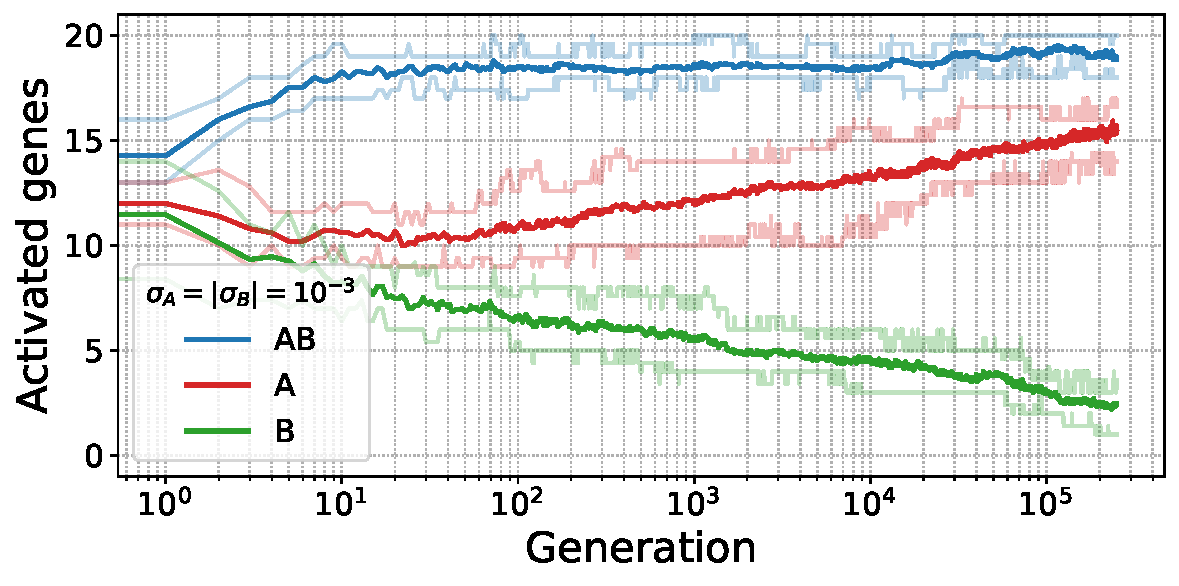
\includegraphics[width=0.495\textwidth]{param/sigma/sigma-1e-3/gene_activity_env_A.pdf}
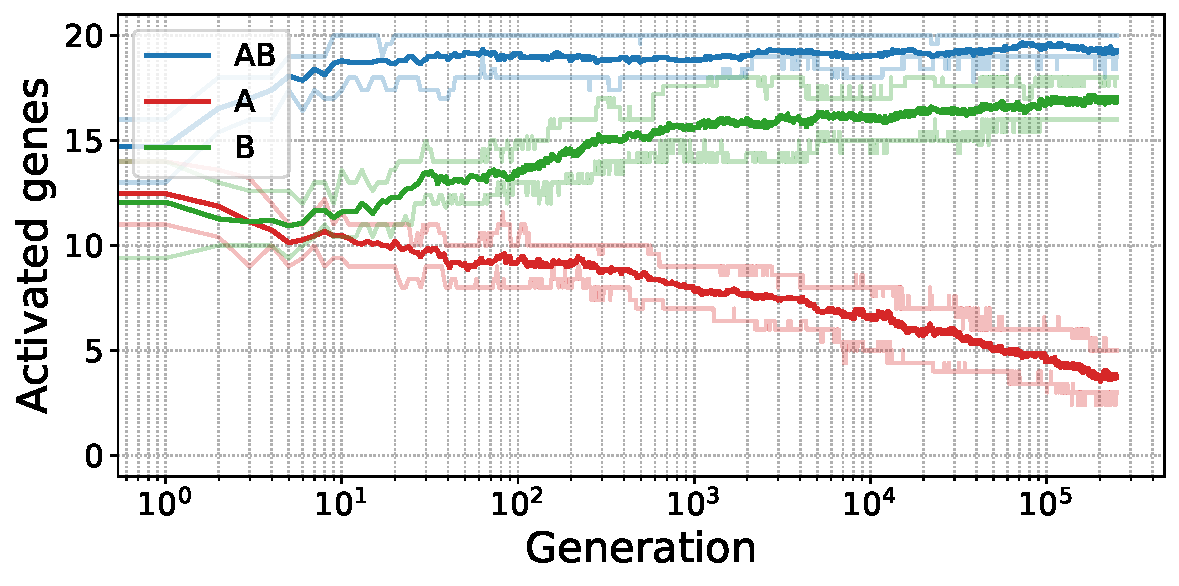
\includegraphics[width=0.495\textwidth]{param/sigma/sigma-1e-3/gene_activity_env_B.pdf}

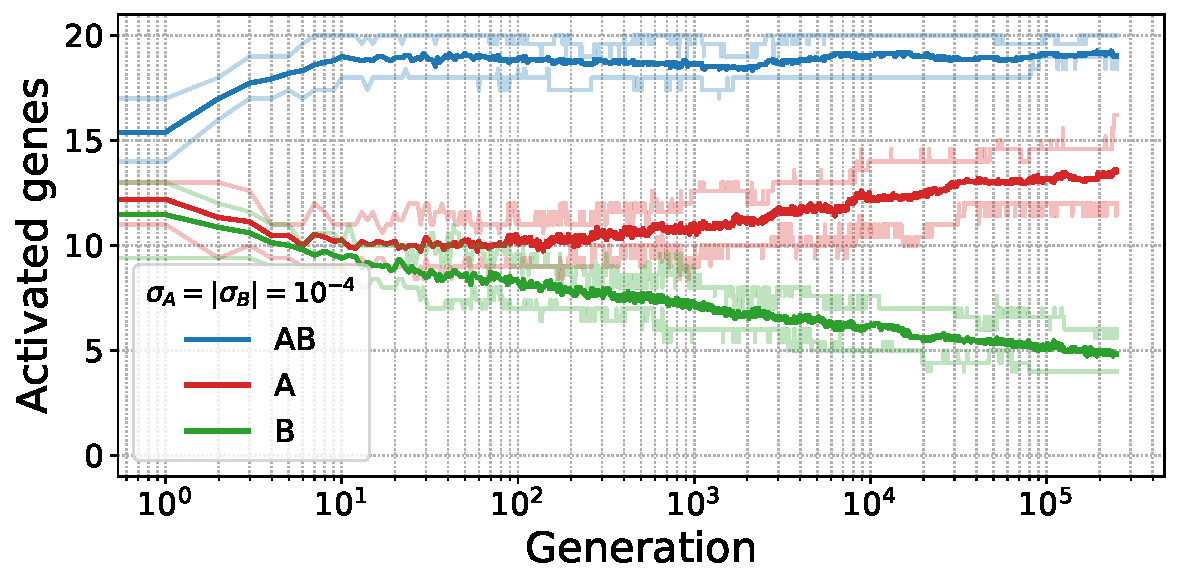
\includegraphics[width=0.495\textwidth]{param/sigma/sigma-1e-4/gene_activity_env_A.pdf}
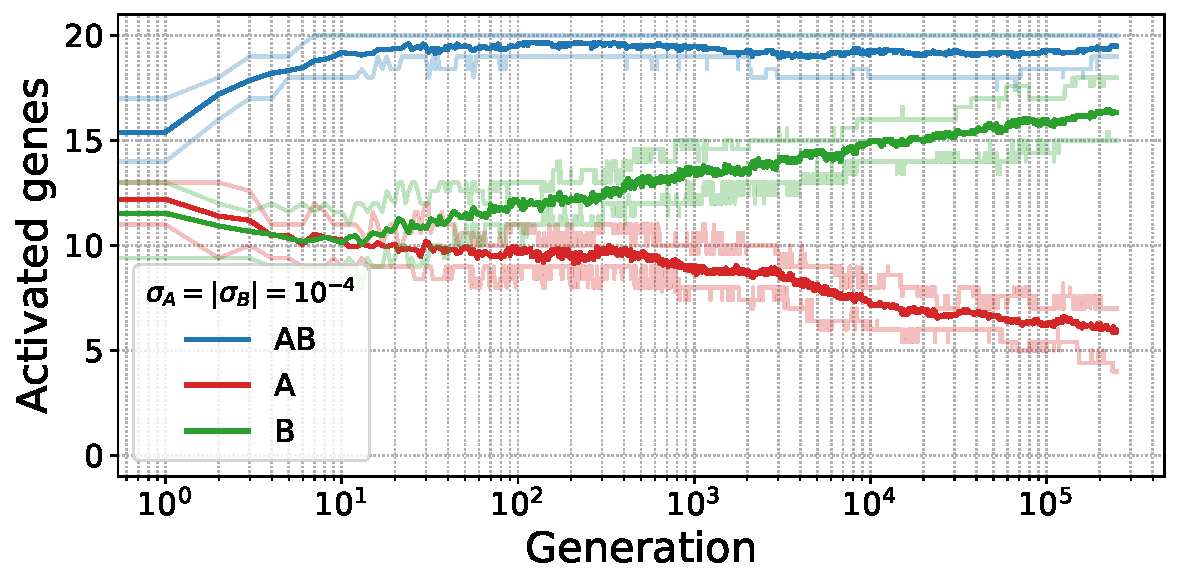
\includegraphics[width=0.495\textwidth]{param/sigma/sigma-1e-4/gene_activity_env_B.pdf}
\caption[Evolution of the number of activated genes in each environment, with decreasing environmental supercoiling shifts]{Evolution of the number of activated genes in environment A (left) and environment B (right), with environmental supercoiling shifts $\sigma_A = 0.001$ and $\sigma_B = -0.001$ (top) and $\sigma_A = 0.0001$ and $\sigma_B = -0.0001$ (bottom).}
\label{fig:param:sigma-activ-by-env}
\end{figure}

Figure~\ref{fig:param:sigma-activ-by-env} shows the evolution of the number of activated genes by type in each environment, with environmental shifts in supercoiling 10 times smaller than the main run (top) and 100 times smaller (bottom), for 250,000 generations.
In both cases, differentiated gene expression patterns evolve, although evolution seems to be slower when $\sigma_A$ and $\sigma_B$ are 100 times smaller than in the main run.
The evolution of different gene expression levels as a response to changes in supercoiling is therefore sensitive even to very small perturbations.
This reinforces the plausibility of the hypothesis that DNA supercoiling can be used as an environmental sensory device for the regulation of gene expression.

\begin{figure}
\centering
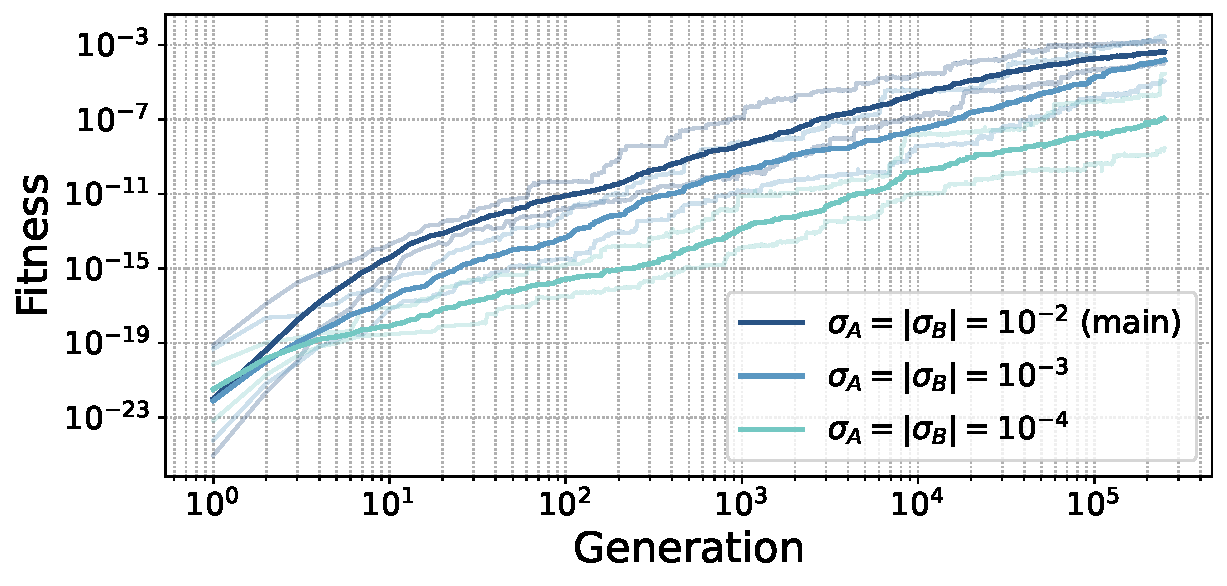
\includegraphics[width=0.75\textwidth]{param/sigma/fitness_all_with_main.pdf}
\caption[Average fitness during evolution, with decreasing environmental supercoiling shifts]{Average fitness during evolution, with environmental shifts in supercoiling $\sigma_A = 0.001$ and $\sigma_B = -0.001$ (10 times smaller than in the main run) and $\sigma_A = 0.0001$ and $\sigma_B = -0.0001$ (100 times smaller than the main run).}
\label{fig:param:sigma-fitness}
\end{figure}

Figure~\ref{fig:param:sigma-fitness} shows the evolution of the average fitness of the best individual in each replicate, for each pair of environmental supercoiling values.
It confirms the results seen in the previous figure: fitness keeps increasing throughout the simulation in all cases, but more slowly when the environmental perturbation is the smallest.

\begin{figure}
\centering
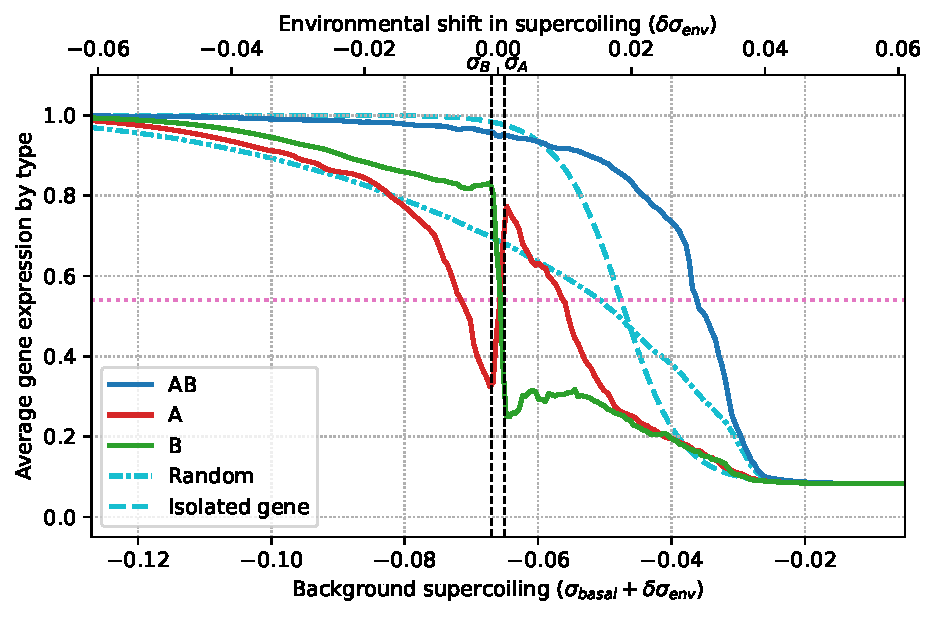
\includegraphics[width=0.9\textwidth]{param/sigma/sigma-1e-3/activity_sigmas_avg.pdf}
\caption[Average gene expression as a function of background supercoiling, with an absolute environmental supercoiling shift of 0.001]{Average gene expression as a function of background supercoiling, with environmental supercoiling shifts $\sigma_A = 0.001$ and $\sigma_B = -0.001$.}
\label{fig:param:sigma-1e-3-activ-by-sigma}
\end{figure}

Figure~\ref{fig:param:sigma-1e-3-activ-by-sigma} shows the average gene expression per gene type as a function of background supercoiling, for the best individuals at the end of evolution with environmental shifts in supercoiling of $\sigma_A = 0.001$ and $\sigma_B = -0.001$.
Even though the difference between the two environments is 10 times smaller than in the main run, \emph{A} genes are still able to evolve a relaxation-activated phenotype, and \emph{B} genes are still able to quickly transition from high activation to high inhibition in a much shorter range of supercoiling values.

\begin{figure}
\centering
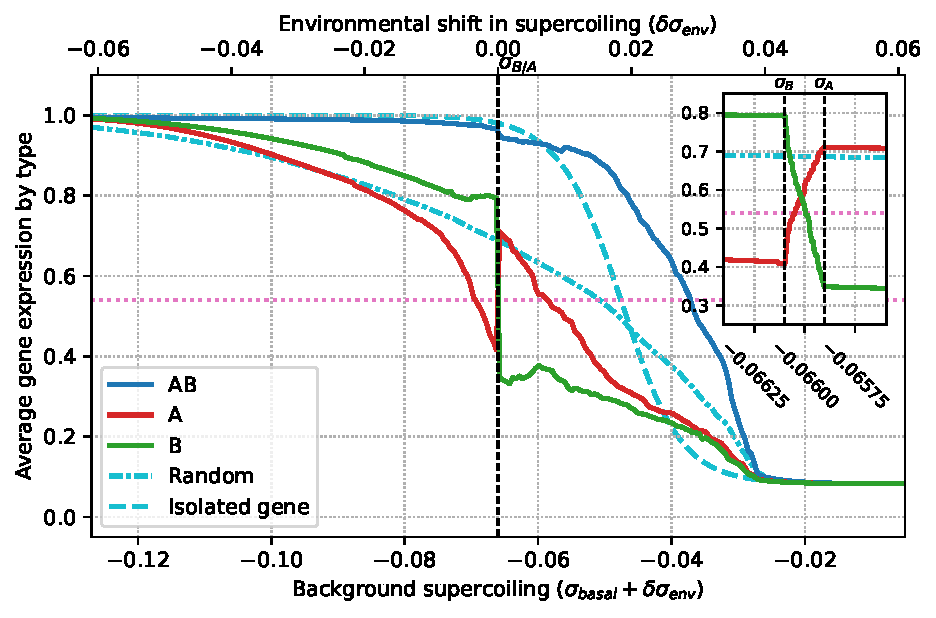
\includegraphics[width=0.9\textwidth]{param/sigma/sigma-1e-4/activity_sigmas_avg.pdf}
\caption[Average gene expression as a function of background supercoiling, with an absolute environmental supercoiling shift of 0.0001]{Average gene expression as a function of background supercoiling, with environmental supercoiling shifts $\sigma_A = 0.0001$ and $\sigma_B = -0.0001$.
The inset at the top right of the figure shows a 150x zoom on supercoiling shift values near zero.}
\label{fig:param:sigma-1e-4-activ-by-sigma}
\end{figure}

Figure~\ref{fig:param:sigma-1e-4-activ-by-sigma} similarly shows average gene expression per gene type as a function of background supercoiling, this time with environmental supercoiling shifts $\sigma_A = 0.0001$ and $\sigma_B = -0.0001$.
Strikingly, \emph{A} genes and \emph{B} genes are still able to evolve different expression levels in the two environments, even though they are 100 times closer than in the original experiment.
Even when the environments have an effect that is around 100 times smaller than the transcription-generated supercoiling (see Figure~\ref{fig:ploscb:genomes} for an example genome and the associated transcription-generated supercoiling values), the gene regulatory networks that evolve in the simulations are still able to separate the different environments and lead gene expression levels to very different states.

\FloatBlock


\section{Number of Genes}
\label{sec:param:300-genes}

All the simulations presented up to now were run with $n = 60$ genes on the genomes of individuals.
Although genes in our model correspond to transcriptional units, and could describe operons that contain multiple genes, this number remains much lower than the real number of genes in bacteria, which ranges from the 482 protein-coding genes found in \emph{Mycoplasma genitalium}, the bacteria with the smallest-known genome~\citep{glass2006}, up to over 9,000 predicted genes in \emph{Sorangium cellulosum}~\citep{schneiker2007}.
At first sight, increasing the total number of genes in the model should not qualitatively change the simulation results, as with a genome size of 60, genes already only interact via the transcription-supercoiling coupling with a small proportion of the genome.
In order to verify this hypothesis, I ran simulations with $n = 300$ genes.
As the algorithmic complexity of the \emph{EvoTSC} scales quadratically with the number of genes, the simulations were run for 100,000 generations only, but already show qualitative results by that time.

\begin{figure}[H]
\centering
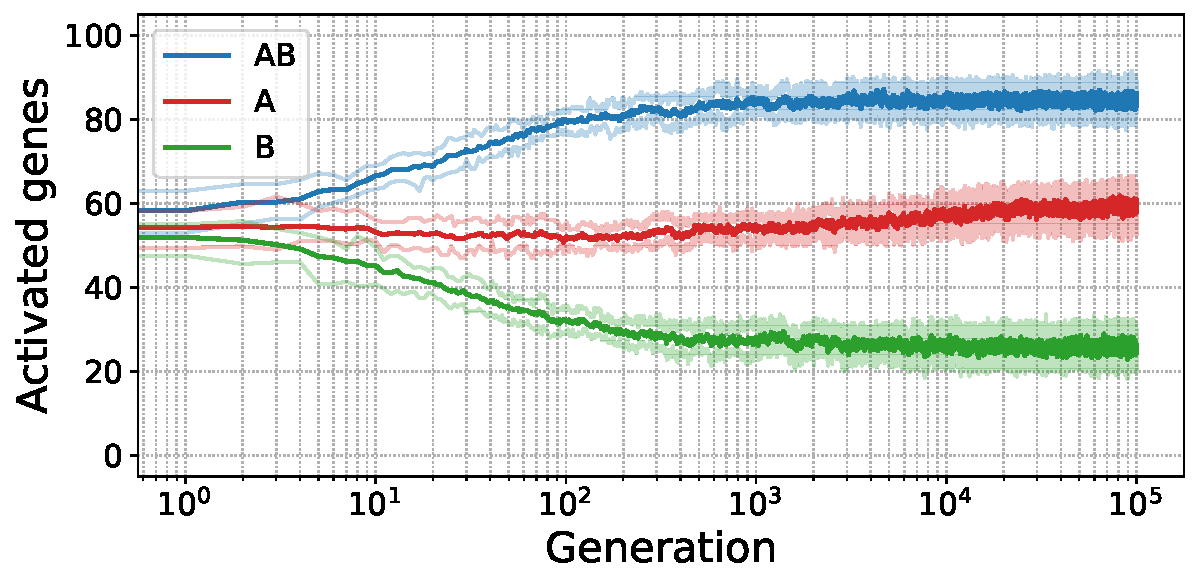
\includegraphics[width=0.495\textwidth]{param/300-genes/gene_activity_env_A.pdf}
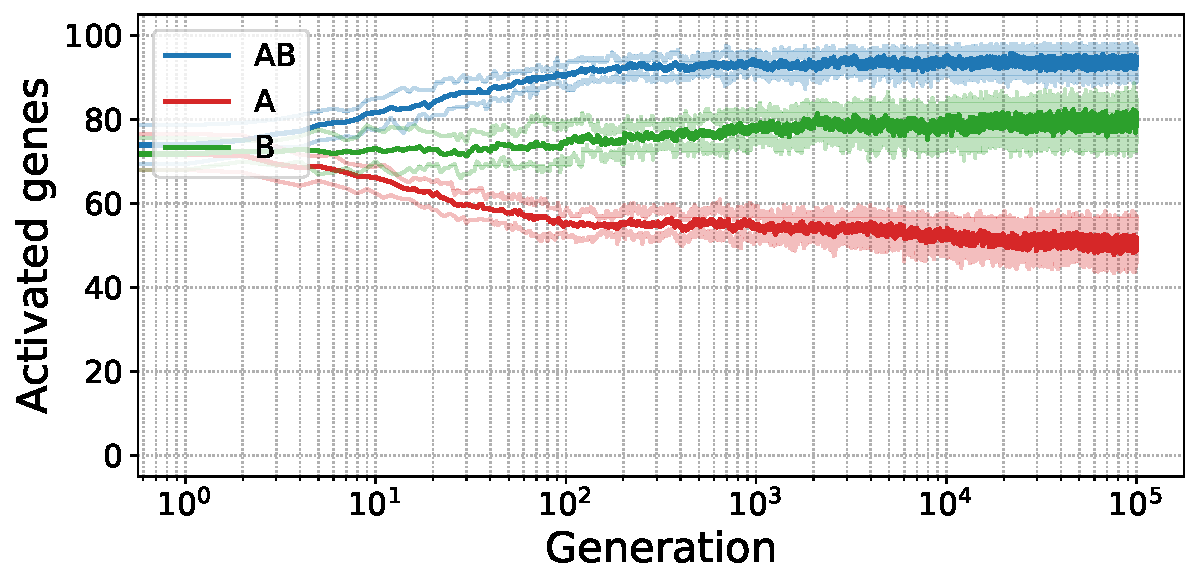
\includegraphics[width=0.495\textwidth]{param/300-genes/gene_activity_env_B.pdf}
\caption[Evolution of the number of activated genes in each environment, with a 300-gene genome]{Evolution of the number of activated genes in environment A (left) and environment B (right), with a genome containing 300 genes.}
\label{fig:param:300genes-activ-by-env}
\end{figure}

Figure~\ref{fig:param:300genes-activ-by-env} shows the evolution of the number of activated genes of each type in each environment, for populations of individuals with a 300-gene genome, for 100,000 generations.
Differentiated expression levels in each environment evolve for \emph{AB} and \emph{B} genes, but the average number of activated \emph{A} genes is only of 60 out of 100 in environment A, and 45 \emph{A} genes are wrongly activated in environment B.
While these simulations lasted only for 100,000 simulations, these evolutionary trajectories are already different from the ones taken by the main run (in Figure~\ref{fig:ploscb:gene_activity_by_env}).

\begin{figure}[H]
\centering
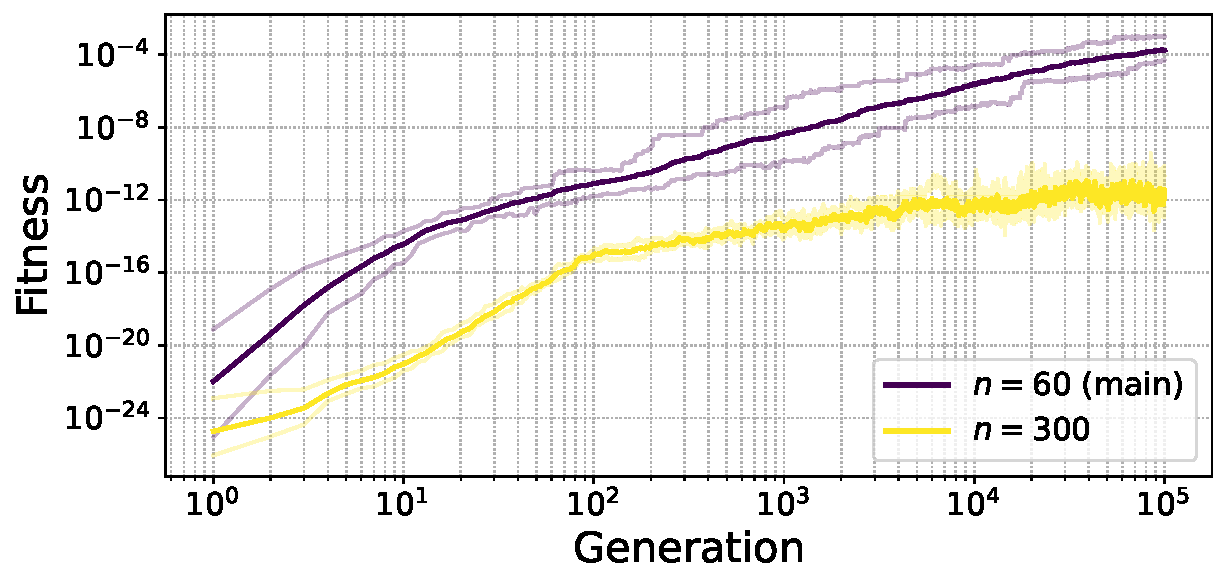
\includegraphics[width=0.75\textwidth]{param/300-genes/fitness_all_with_main.pdf}
\caption[Average fitness during evolution, with a 300-gene genome]{Average fitness during evolution, with a 300-gene genome.}
\label{fig:param:300gene-fitness}
\end{figure}

Figure~\ref{fig:param:300gene-fitness} shows the evolution of the average fitness of the best individual in each replicate of the simulations with 300 genes per individual, compared to the main run.
As expected from the number of activated genes in each environment presented in Figure~\ref{fig:param:300genes-activ-by-env}, the fitness of the runs with 300 genes is consistently lower than the fitness of the main runs, and seems to converge to a much lower value by the end of the 100,000 generations of evolution.

\begin{figure}[H]
\centering
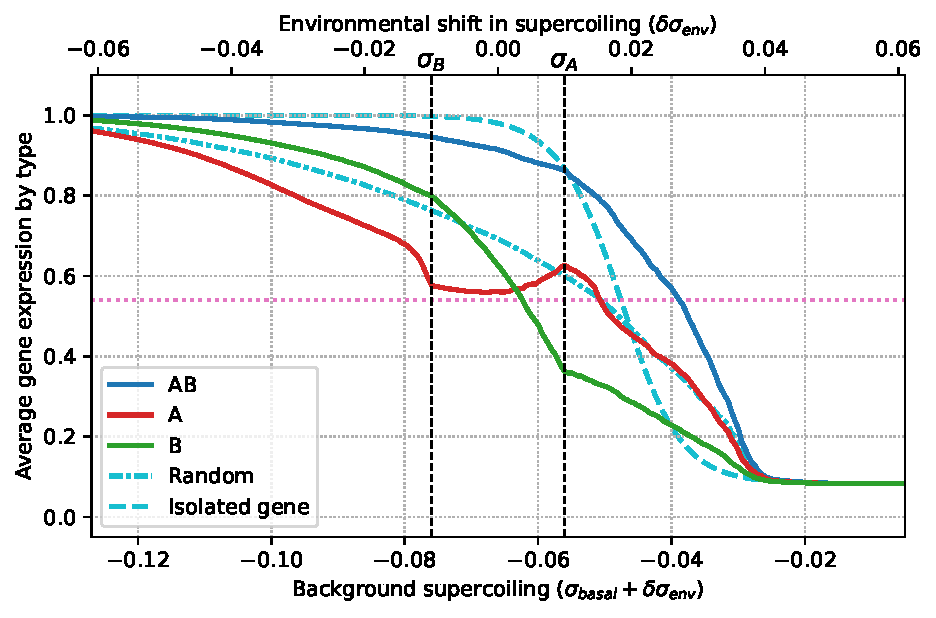
\includegraphics[width=0.9\textwidth]{param/300-genes/activity_sigmas_avg.pdf}
\caption[Average gene expression as a function of background supercoiling, with a 300-gene genome]{Average gene expression by type as a function of background supercoiling, with a 300-gene genome.}
\label{fig:param:300genes-activ-by-sigma}
\end{figure}

Figure~\ref{fig:param:300genes-activ-by-sigma} shows the average expression of genes, separated by type, to the background supercoiling level.
Similarly to the simulation with a 10 kb intergenic distance, \emph{A} genes do not seem to meaningfully evolve a relaxation-activated phenotype by the end of the simulations.
With 300 genes, the response of each gene type looks to diverge less from the behavior of genes on a random genome than for the other simulations presented above.

This could indicate that the fitness landscape for these populations is more rugged than in the other cases.
As the end points of genomic inversions are chosen at random, the average size of an inversion is of half the genome with all parameter values, but the absolute number of genes between the end points of the inversion changes with the number of genes on the genome.
A possible hypothesis to explain the difference in evolutionary trajectories could therefore be that, in larger genomes, both end points of an inversion are more rarely part of the same gene regulatory network, which could make it more difficult for selection to tune these networks as precisely as in the smaller genomes.

\FloatBlock


\section{Mutable Intergenic Size}
\label{sec:param:evolve-intergene}

The last set of simulations presented in this chapter tackle the exploration of the model in a different direction, by introducing a new mutational operator.
We saw previously in Section~\ref{sec:param:mean-intergene} that the evolution of differentiated gene expression patterns is robust to variations in the mean distance between genes on the genome, with the clearest patterns (and, correspondingly, highest fitness) evolving at a mean intergenic distance of 1 kb (in Figure~\ref{fig:param:mean-intergene-activ-by-env}, middle row).
In order to see whether the fitness peak at high intergenic distances would be reachable from their original values, I introduced a new mutational operator which allows intergenic distances to evolve, through the addition or deletion of a small number of bases (indels).

In order to perform an indel in the model, we first pick a number of base pairs to add or delete, by drawing from a normal distribution $\mathcal{N}(0, s^2)$, with $s^2 = $ 10.
Then, we draw uniformly at random a gene, and add or remove the corresponding number of bases from the intergenic section starting at that gene \textbf{Ça devrait plutôt être uniforme selon la longueur des sections intergéniques -- note: ça n'a pas l'air de changer cf. figures}.
If the intergenic section is too small to delete the chosen number of base pairs, we try drawing another gene at random, before giving up after a certain number of tries.
For these simulations, I ran 15 replicates for 1,000,000 generations (as in the main runs in Chapter~\ref{chap:ploscb}), in order to give the mean intergenic distance the time to converge, and started from an initial value of 125 bp, as in the main simulations.

\begin{figure}
\centering
  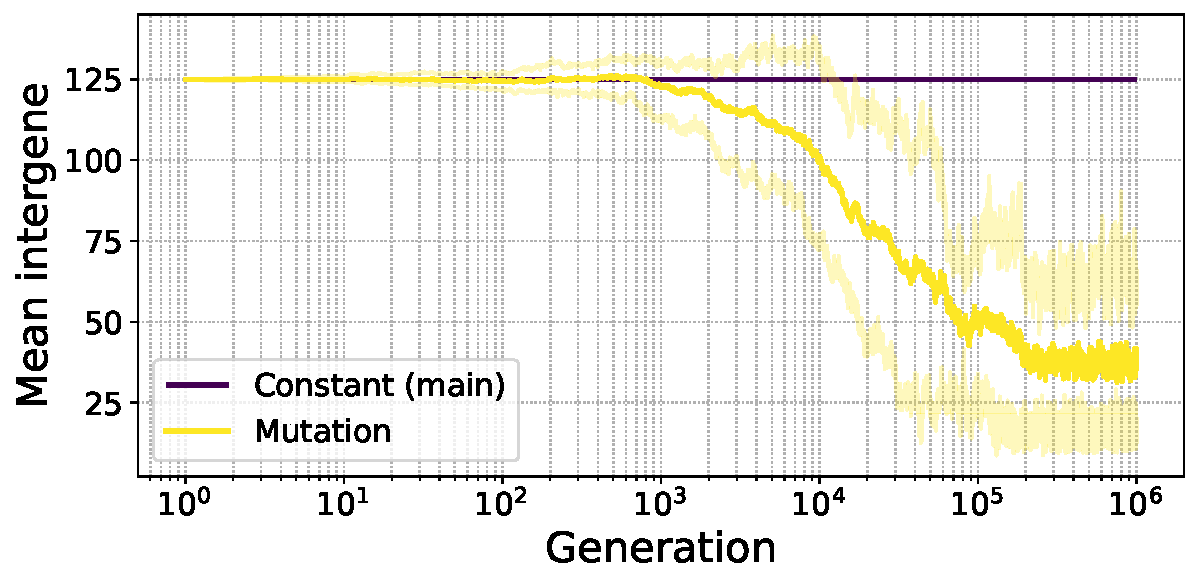
\includegraphics[width=0.75\textwidth]{param/evolve-intergene/intergenic_size_all.pdf}
\caption[Average intergenic size during evolution, with intergenic distance mutations]{Average intergenic distance during evolution with indels, compared with the average intergenic distance in the main run.}
\label{fig:param:evolve-intergene-intergene}
\end{figure}

Figure~\ref{fig:param:evolve-intergene-intergene} show the evolution of the mean intergenic distance, averaged over he best individual of each replicate, at every generation, compared to the initial value of 125 bp.
Oppositely to what was expected, the average intergenic distance actually decreases during evolution, and seems to converge to a value of around 40 bp.
There therefore seems to be a selection pressure towards reducing intergenic distances, when they are allowed to evolve.

\begin{figure}[H]
  \centering
  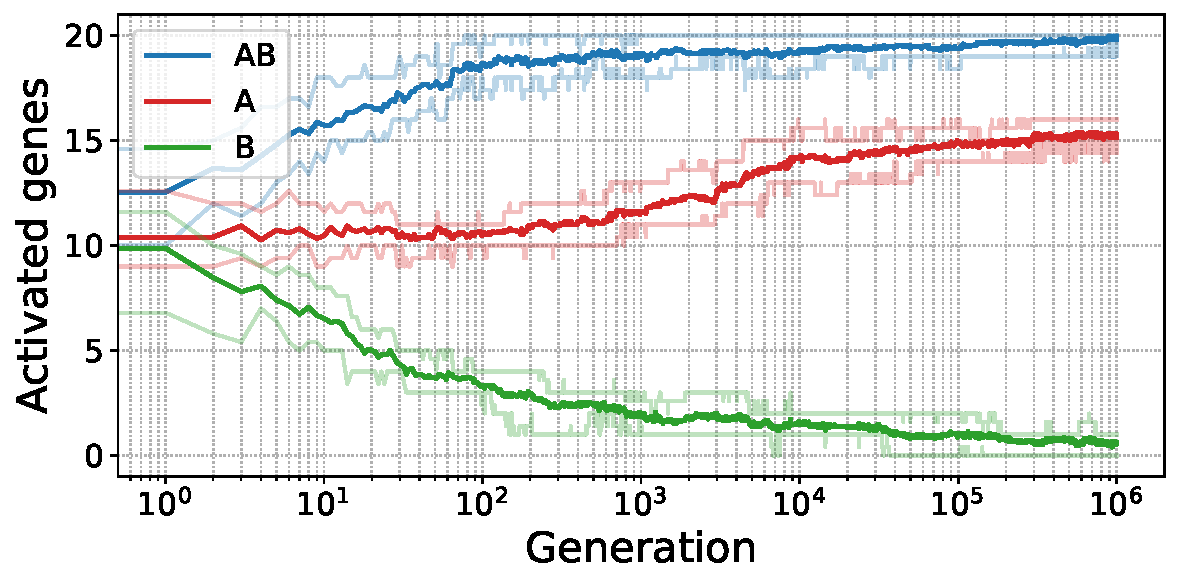
\includegraphics[width=0.495\textwidth]{param/evolve-intergene/gene_activity_env_A.pdf}
  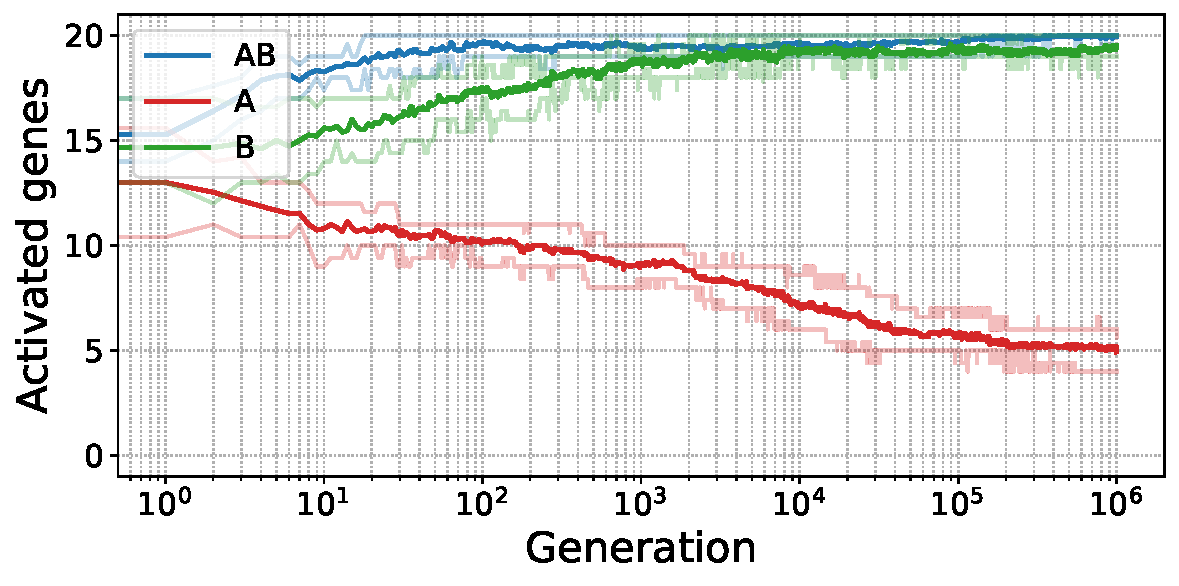
\includegraphics[width=0.495\textwidth]{param/evolve-intergene/gene_activity_env_B.pdf}
  \caption[Evolution of the number of activated genes in each environment, with intergenic distance mutations]{Evolution of the number of activated genes in environment A (top) and environment B (bottom), with intergenic distance mutations.}
  \label{fig:param:evolve-intergene-activ-by-env}
\end{figure}

Figure~\ref{fig:param:evolve-intergene-activ-by-env} shows the evolution of the number of activated genes of each type, in each environment.
As in the main run, differentiated expression levels evolve in the two environments, with around 75\% of \emph{A} genes activated in environment A and 75\% of \emph{A} inhibited in environment B.

\begin{figure}
\centering
  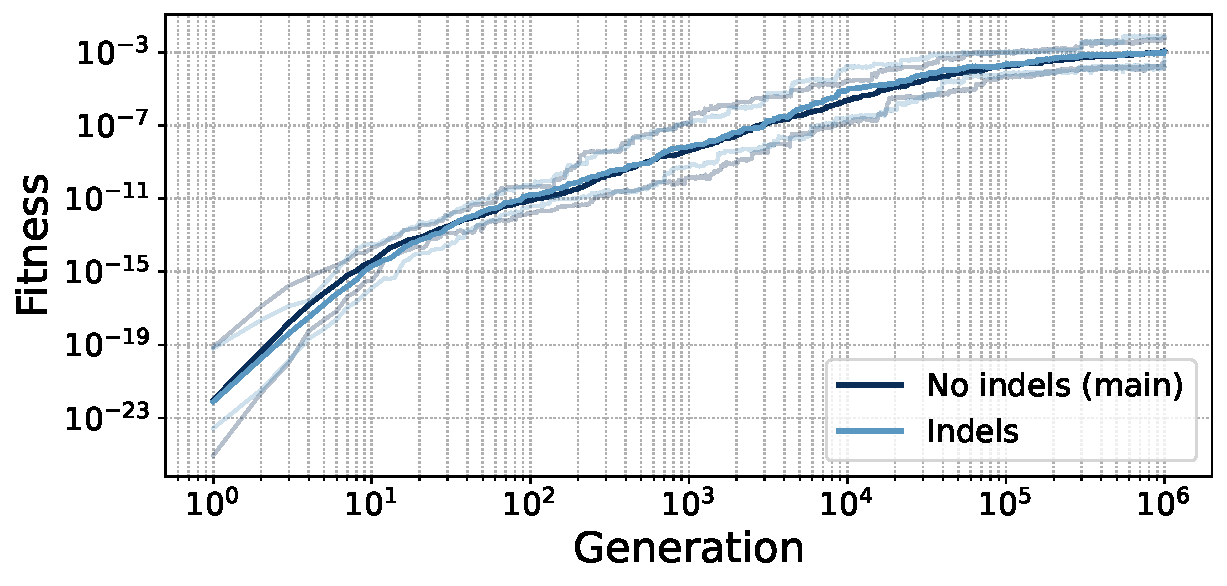
\includegraphics[width=0.75\textwidth]{param/evolve-intergene/fitness_all_with_main.pdf}
\caption[Average fitness and intergenic size during evolution, with intergenic distance mutations]{Fitness and average genome size during evolution, with intergenic distance mutations.}
\label{fig:param:evolve-intergene-fitness}
\end{figure}

Figure~\ref{fig:param:evolve-intergene-fitness} shows the average fitness during evolution of the individuals in the simulations with mutations in the intergenic distances, compared with the main simulations.
As for the runs with an intergenic distance of 10 bp (in Figure~\ref{fig:param:mean-intergene-fitness}), evolution progresses extremely similarly to the main runs.

\begin{figure}[H]
\centering
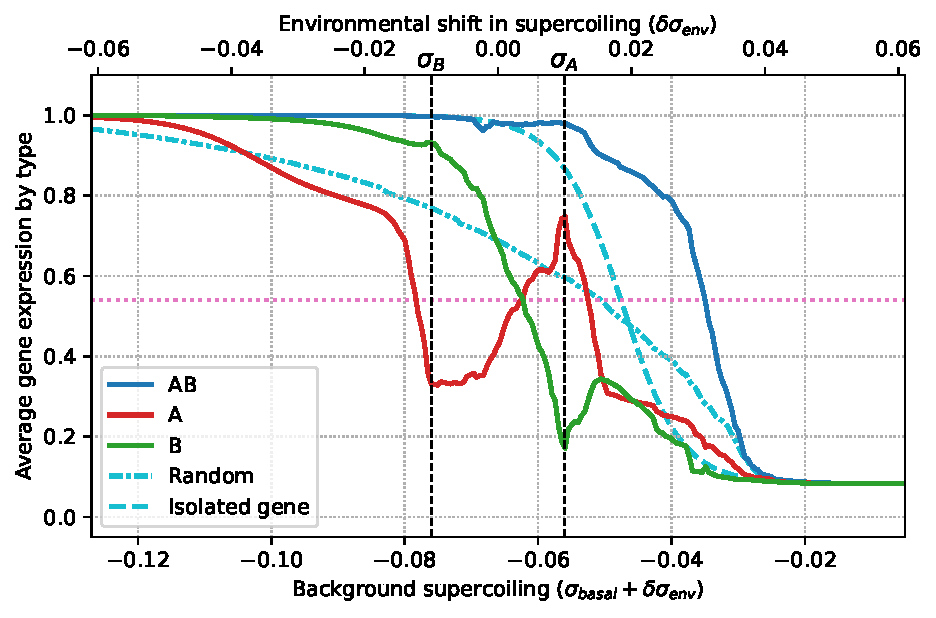
\includegraphics[width=0.9\textwidth]{param/evolve-intergene/activity_sigmas_avg.pdf}
\caption[Average gene expression as a function of background supercoiling, with intergenic distance mutations]{Average gene expression by type as a function of background supercoiling, with intergenic distance mutations.}
\label{fig:param:evolve-intergene-activ-by-sigma}
\end{figure}

Finally, Figure~\ref{fig:param:evolve-intergene-activ-by-sigma} shows gene activity per type as a function of background supercoiling, for the simulations with mutable intergenic distances.
As expected, we can see that \emph{A} genes display a relaxation-activated phenotype.

It therefore seems that, even though evolving towards higher intergenic distances would allow populations to reach greater fitnesses, there is a stronger selection pressure that keeps intergenic distances low.
This suggests that the fitness valley that has to be crossed in order to reach higher intergenic distances is too wide, or too deep, to cross with the parameters that we chose for the indel mutational operator.


%\begin{figure}
%\centering
%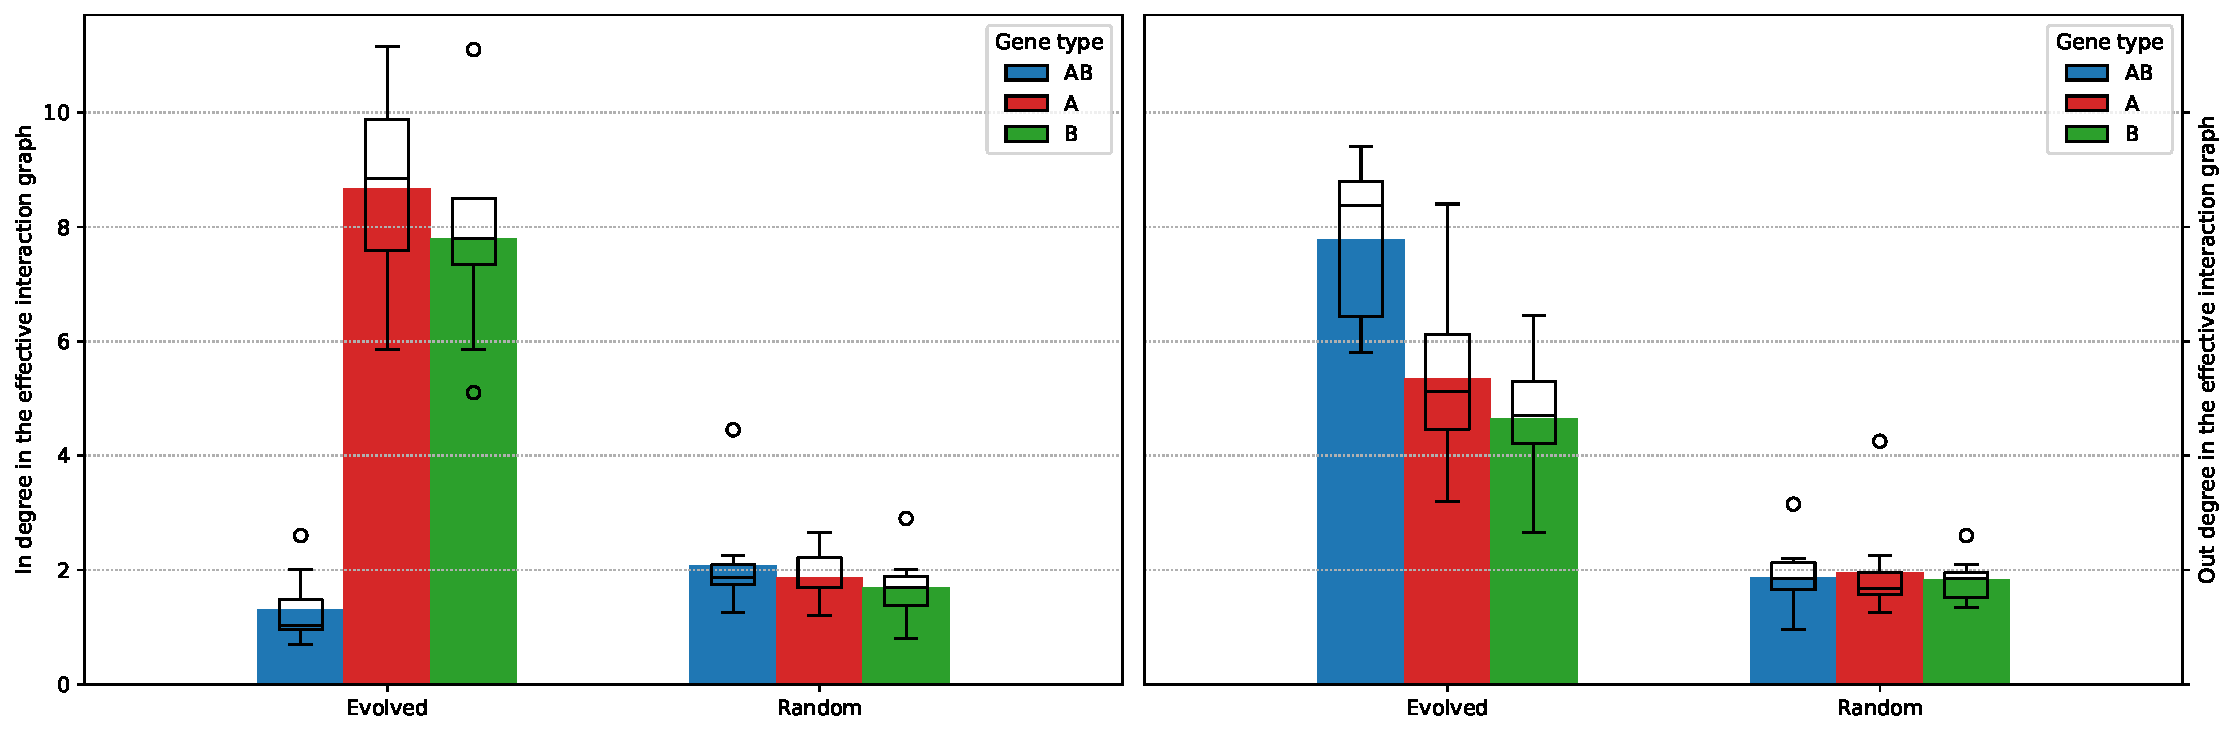
\includegraphics[width=\textwidth]{param/evolve-intergene/effective_graph_combined_degree.pdf}
%\caption{Effective graph degrees at the end of evolution with intergenic distance mutations.}
%\end{figure}

\section{Discussion}

The simulations that I carried out with the parameter values presented above show that the results obtained with the model are quite robust, as differentiated gene expression by type and environment evolve over a wide range of biologically relevant values.
In particular, results are robust with regard to the size of topological domains, which corresponds to the maximum interaction distance for the transcription-supercoiling coupling and has been measured to different values, to the mean intergenic distance, which depends on the bacterial species, and to the environmental perturbations.
The gene regulatory networks that evolve in the model can indeed differentiate between environments that create much smaller levels of supercoiling than transcription itself.

The fact that genomes with a higher number of genes or intergenic distances (above 10 kb) are not able to evolve a fitness as high as the smaller genomes shows that the topology of the fitness landscape inherent to the model changes with the value of these parameters.
The number of possible mutations using the mutational operator of genomic inversions indeed scales quadratically with the number of base pairs on the genome, thereby directing the number of possible genotypes that can be explored in a given number of generations with a constant number of individuals.
In order to explore this effect, it would be interesting to run additional simulations in which every length-related parameter  (maximum interaction distance, mean intergenic distance, and gene length) would be scaled down down by the same factor, as this would allow to control the number of mutations available and therefore the speed of evolution, but should not in principle affect the biological relevance of the model.

Finally, introducing indels as an additional mutational operator also reveals non-trivial evolutionary characteristics of the simulations.
Indeed, the maximum fitness obtainable with a 1 kb intergenic distance is not reached by the simulations, which instead converge to a a very low average intergenic distance.
It would be interesting to explore different initial values for this parameter and see whether they also converge towards this low value, or if there is a threshold above which the fitness peak at high intergenic distances is reachable.
A possible hypothesis to explain the attraction to the low mean intergenic distance could be once again related to the genomic inversions, through selection for robustness: If larger genomes have descendants that more frequently have lower fitness because of deleterious inversions than smaller genomes, there can be a selection pressure towards these smaller genomes, even though they have a lower absolute fitness; this could be measured experimentally by measuring the average fitness of a large number of descendants of evolved individuals in the different simulations.
